\documentclass[class=report, crop=false, 12pt,a4paper]{standalone}
\usepackage{enumitem}
\usepackage{multicol}
\usepackage{graphicx}
\usepackage{float}
\usepackage{amsmath}
\usepackage{amssymb}
\usepackage{mathtools}
\usepackage{siunitx}
\usepackage{commath}
\usepackage{array}
\usepackage{natbib}
\usepackage{tikz}
\usepackage[a4paper,width=150mm,top=25mm,bottom=25mm]{geometry}
\usetikzlibrary{positioning, fit, calc}   
\tikzset{block/.style={draw, thick, text width=3cm ,minimum height=1.3cm, align=center},   
line/.style={-latex}     
}  
\setlength{\parindent}{0pt}
\begin{document}
\begin{center}
    24/11/2020
\end{center}
\section*{Boundary layer theory (Prandtl)}
The flow domain can be subdivided into two parts:
\begin{itemize}
  \item \textbf{Irrotational flow region}, outside of the boundary layer, Bernoulli equation, potential flow and stream function apply
  \item \textbf{Boundary layer} where all vorticity is confined, The friction shear at the airfoil surface acts as a source of vorticity. 
\end{itemize}
\begin{figure}[H]
  \centering
  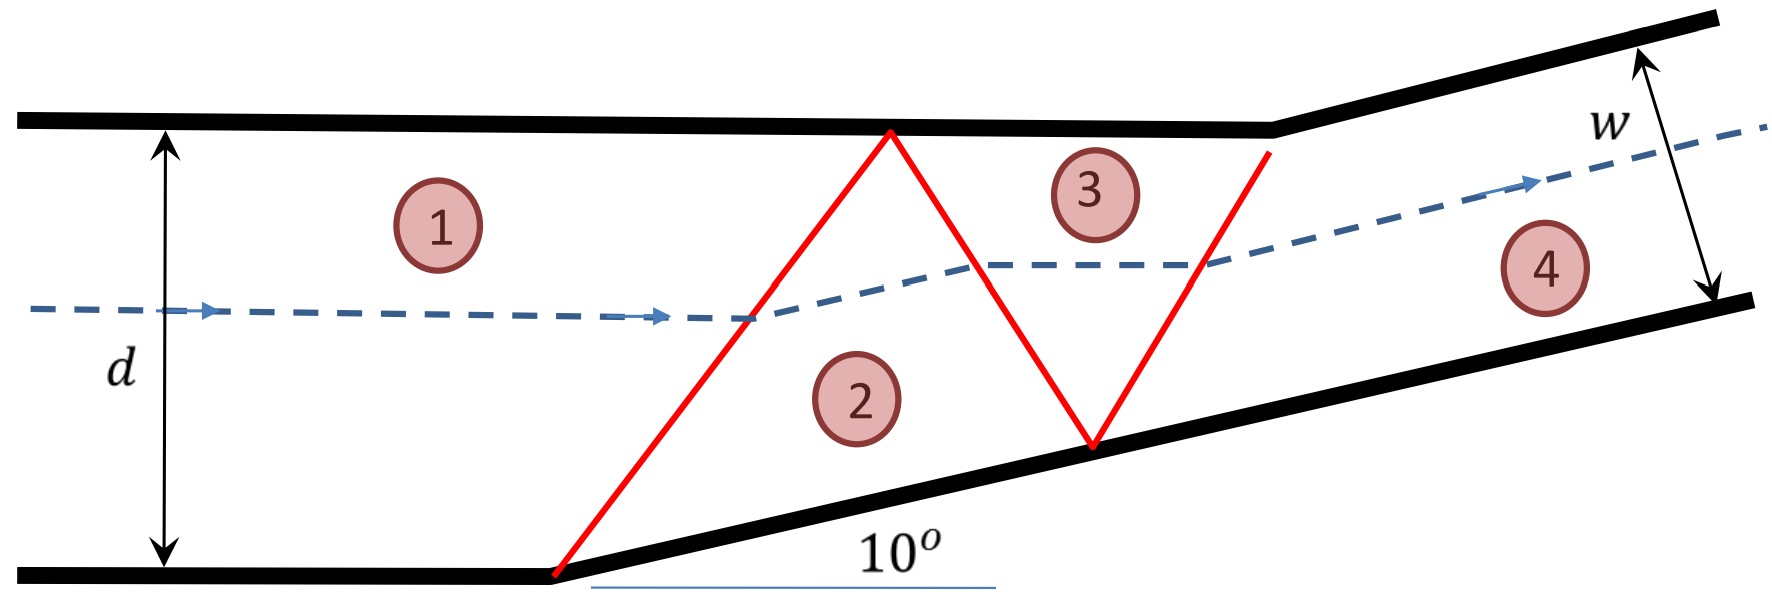
\includegraphics[width = 0.8 \textwidth]{../img/diagram48.png}
\end{figure}
\section{Boundary layer concept}
Immediately adjacent to a solid surface, the fluid particles are slowed by the strong shear force between the fluid particles and the surface. This relatively slower moving layer of fluid is the boundary layer.
\begin{figure}[H]
  \centering
  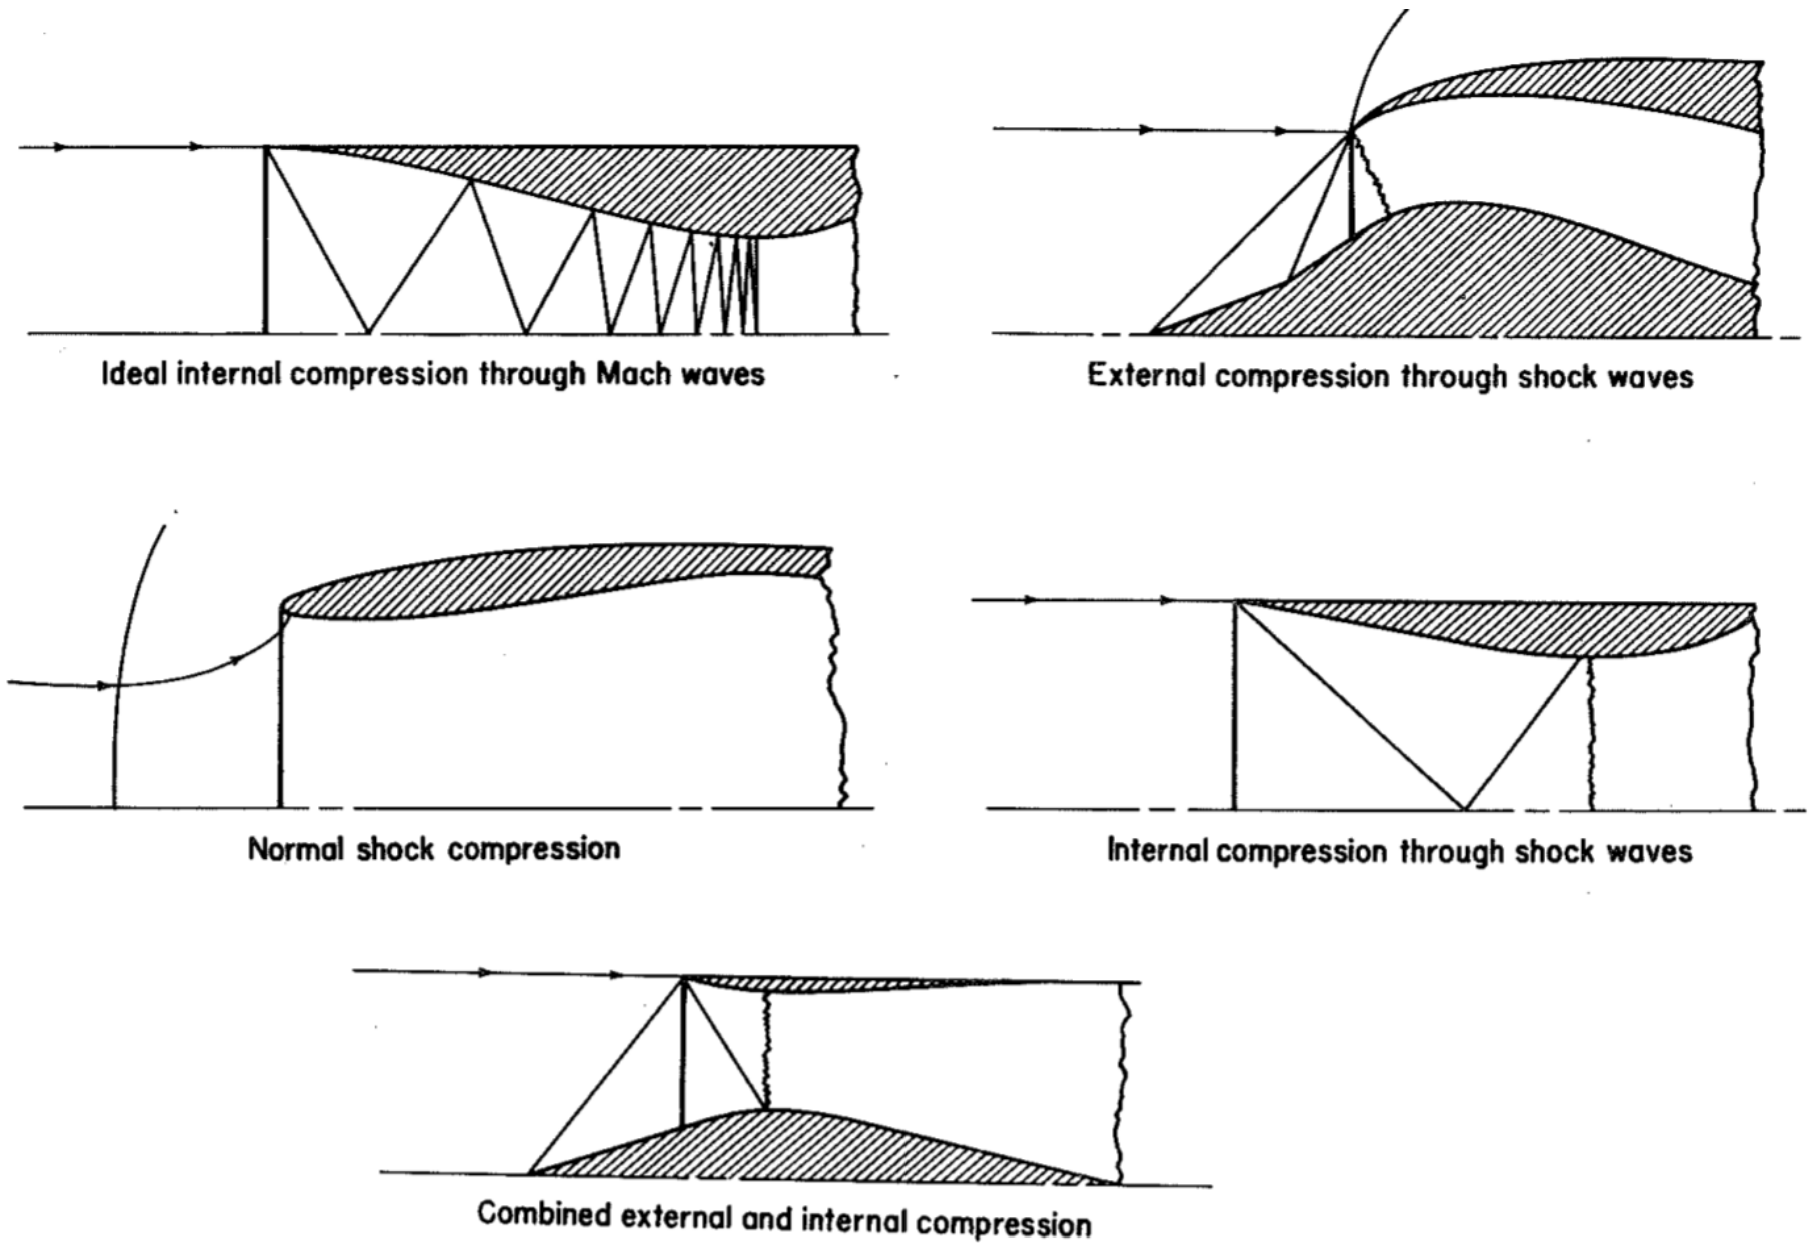
\includegraphics[width = 0.8 \textwidth]{../img/diagram49.png}
  \caption{In turbulent flow, you have a higher shear stress due to the higher velocity close to the boundary. This produces more frictional drag against the motion of the solid surface. ($\tau = \mu \frac{\partial u}{\partial y}$)}
\end{figure}
\section{Boundary layer theory}
Prandtl's concept of the boundary layer in high $Re$ flow is that although viscous forces can be considered small, their effects are not negligible.
\begin{figure}[H]
  \centering
  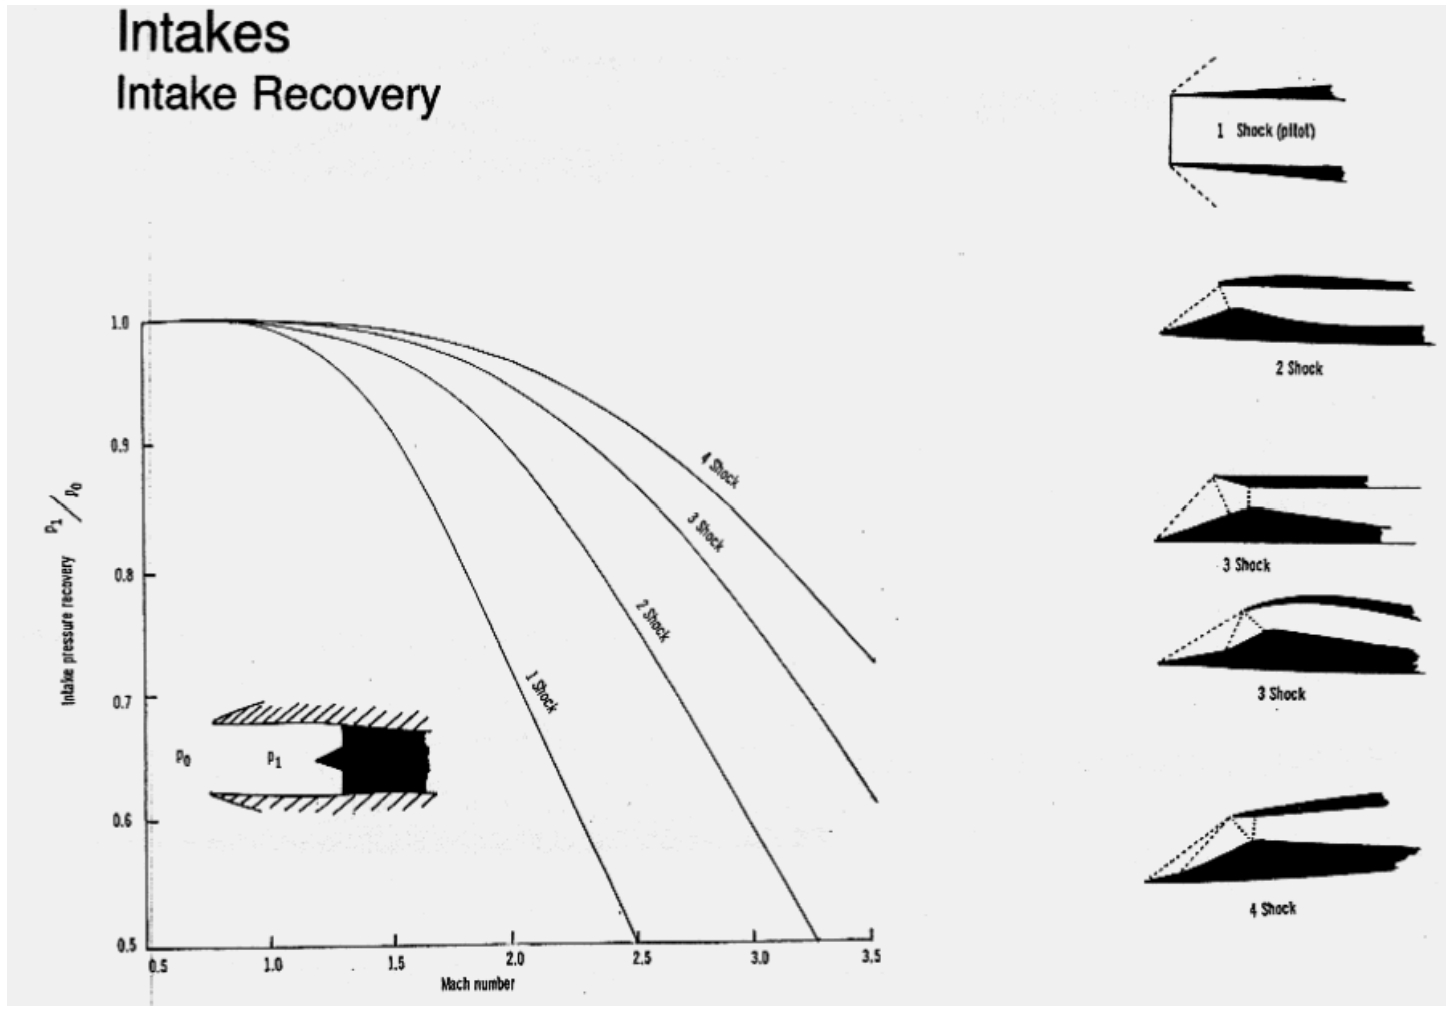
\includegraphics[width = 0.8 \textwidth]{../img/diagram50.png}
\end{figure}
Let us see what happens when we consider the Navier stokes equations for a steady - 2D flow with $Re >> 1$. Continuity equation (conservation of mass):
\begin{align}
  \frac{\partial u}{\partial x} + \frac{\partial v}{\partial y} = 0
\end{align}
Conservation of momentum equations:
\begin{align}
  \textrm{x-direction: } u\frac{\partial u}{\partial x} + v \frac{\partial u }{\partial y} &= - \frac{1}{\rho} \frac{\partial p}{\partial x} + \nu \left(\frac{\partial^2 u}{\partial x^2} + \frac{\partial^2 u}{\partial y^2}\right)\\
  \textrm{y-direction: } u \frac{\partial v}{\partial x} + v\frac{\partial v}{\partial y} &= -\frac{1}{\rho}\frac{\partial p}{\partial y} + \nu \left(\frac{\partial^2 v}{\partial x^2} + \frac{\partial^2 v}{\partial y^2}\right)
\end{align}
Remember that:
\begin{equation}
  Re = \frac{U_\infty L}{\nu}
\end{equation}
Where $L$ is the length of the airfoil being analysed, $U_\infty$ is the velocity of the free stream and $\nu$ the kinematic viscosity. Inside the boundary layer, one thing we can assume that the inertial forces and the viscous forces are comparable, because viscous diffusion is large and of the same order of magnitude of the inertial terms. Therefore:
\begin{align}
  \frac{u\frac{\partial u}{\partial x}}{\nu \frac{\partial^2 u}{\partial y^2}} \approx 1
\end{align}
We need to exploit this relationship in order to derive an expression for $\delta$ in comparison to $L$. Some approximations we can make below are:
\begin{align}
  u &\approx U_\infty\\
  x &\approx L \rightarrow \frac{\partial}{\partial x} \propto \frac{1}{L}\\
  y &\approx \delta \rightarrow \frac{\partial}{\partial y} \propto \frac{1}{\delta}
\end{align}
Combining this with our above assumption:
\begin{align}
  \frac{\frac{U_\infty^2}{L}}{\nu \frac{U_\infty}{\delta^2}} &= \frac{\delta^2}{L^2} Re \approx 1\\
  \delta^2 &\approx \frac{L^2}{Re}
\end{align}
Looking at the continuity equation:
\begin{align}
  \frac{\partial u}{\partial x} + \frac{\partial v}{\partial y} &= 0\\
  \frac{U_\infty}{L} + \frac{v}{\delta} &= 0\\
  v &= \frac{\delta}{L}U_\infty\\
  v &= \frac{1}{\sqrt{Re}} U_\infty
\end{align}
(signs were ignored). Looking at the momentum equation in the x-direction:
\begin{align}
  u\frac{\partial u}{\partial x} + v \frac{\partial u }{\partial y} &= - \frac{1}{\rho} \frac{\partial p}{\partial x} + \nu \left(\frac{\partial^2 u}{\partial x^2} + \frac{\partial^2 u}{\partial y^2}\right)\\
  \textrm{First term: } u\frac{\partial u}{\partial x} &\propto \frac{U_\infty^2}{L}\\
  \textrm{Second term: } v\frac{\partial u}{\partial y} &\propto \frac{1}{\sqrt{Re}} \frac{U_\infty}{\delta} U_\infty = \frac{U_\infty^2}{\sqrt{Re}} \frac{\sqrt{Re}}{L} = \frac{U_\infty^2}{L}\\
  \textrm{Fourth term: } \nu \frac{\partial^2 u}{\partial x^2} &\propto \nu \frac{U_\infty}{L^2} = \frac{\nu}{L U_\infty} \frac{U_\infty^2}{L} = \frac{1}{Re} \frac{U_\infty^2}{L}\\
  \textrm{Fifth term: } \nu \frac{\partial^2 u}{\partial y^2} &\propto \nu \frac{I_\infty}{\delta^2} = \frac{\nu}{L U_\infty} \frac{U_\infty^2 L}{\delta^2} = \frac{1}{Re} \frac{U_\infty^2 Re}{L} = \frac{U_\infty^2}{L}
\end{align}
We can see in the fourth term that $Re >> 1$, hence it is neglected i.e. there will not be a viscous term due to the variation of the velocity in the x direction w.r.t x. Looking at the momentum equation in the y-direction:
\begin{align}
  u \frac{\partial v}{\partial x} + v\frac{\partial v}{\partial y} &= -\frac{1}{\rho}\frac{\partial p}{\partial x} + \nu \left(\frac{\partial^2 v}{\partial x^2} + \frac{\partial^2 v}{\partial y^2}\right)\\
  \textrm{First term: } u \frac{\partial v}{\partial x} &\propto U_\infty^2\frac{\delta}{L^2} = \frac{1}{\sqrt{Re}}\frac{U_\infty^2}{L}\\
  \textrm{Second term: } v\frac{\partial v}{\partial y} &\propto \frac{U_\infty^2}{L^2} \frac{\delta^2}{\delta} = \frac{1}{\sqrt{Re}} \frac{U_\infty^2}{L}\\
  \textrm{Fourth term: } \nu \frac{\partial^2 v}{\partial x^2} &\propto \nu \frac{U_\infty \delta}{L} \frac{1}{L^2} = \frac{\nu}{L U_\infty} \frac{U_\infty^2 \delta}{L^2} = \frac{1}{Re} \frac{U_\infty^2}{L\sqrt{Re}} = \frac{1}{\sqrt{Re}^3} \frac{U_\infty^2}{L}\\
  \textrm{Fifth term: } \nu \frac{\partial^2 v}{\partial y^2} &\propto \nu \frac{U_\infty \delta}{L} \frac{1}{\delta^2} = \frac{\nu}{LU_\infty} \frac{U_\infty^2}{\delta} = \frac{1}{Re} \frac{U_\infty^2 \sqrt{Re}}{L} = \frac{1}{\sqrt{Re}} \frac{U_\infty^2}{L}
\end{align}
We see that in the first, second, fourth and fifth terms, $Re >> 1$, hence they are neglected. Let us see what this analysis tells us:
\begin{align}
  \textrm{x-direction: } u\frac{\partial u}{\partial x} + v \frac{\partial u }{\partial y} &= - \frac{1}{\rho} \frac{\partial p}{\partial x} + \nu \frac{\partial^2 u}{\partial y^2}\\
  \textrm{y-direction: } \frac{\partial p}{\partial y} &= 0
\end{align}
\begin{figure}[H]
  \centering
  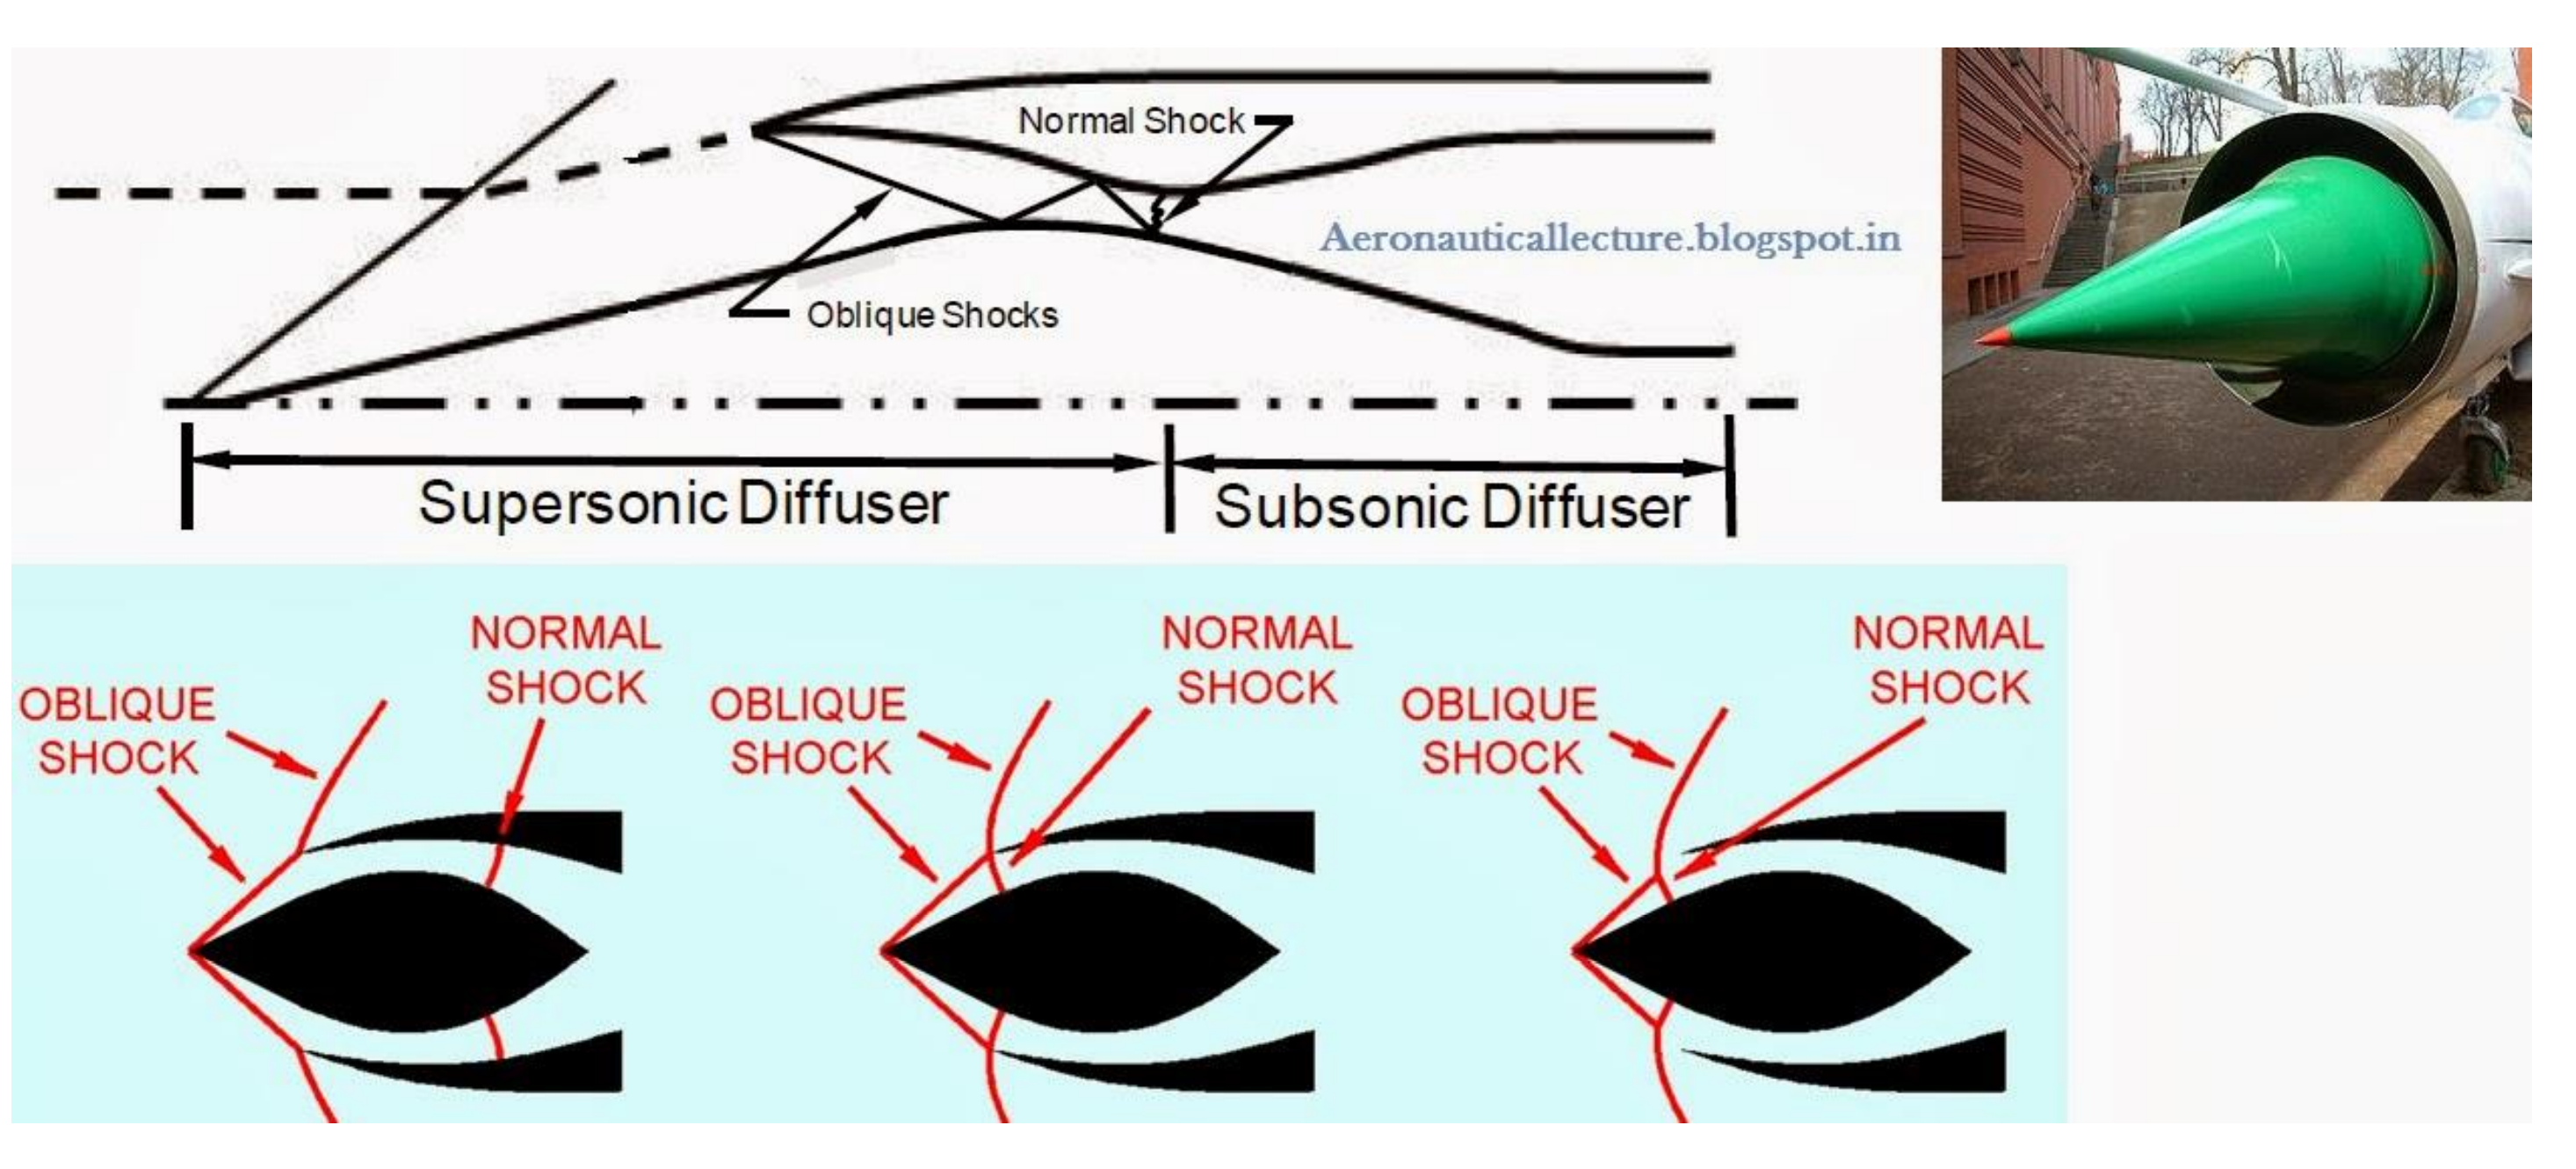
\includegraphics[width = 0.8 \textwidth]{../img/diagram51.png}
\end{figure}
Pressure does not change along thickness of the boundary layer. Therefore I can estimate the pressure outside of the boundary layer using Bernoulli (inviscid flow theory), and then apply that pressure on the body wall. Outside of the boundary layer, we know:
\begin{gather}
  \frac{\partial}{\partial y} = 0 \ \& \ v = 0\\
  U(x) = \frac{\partial U(x)}{\partial x} = \frac{\partial \frac{1}{2}U(x)^2}{\partial x} = -\frac{1}{\rho} \frac{\partial p}{\partial x}\\
  p + \frac{1}{2} \rho U(x)^2 = \textrm{const}
\end{gather}
\section{Flow separation}
\begin{figure}[H]
  \centering
  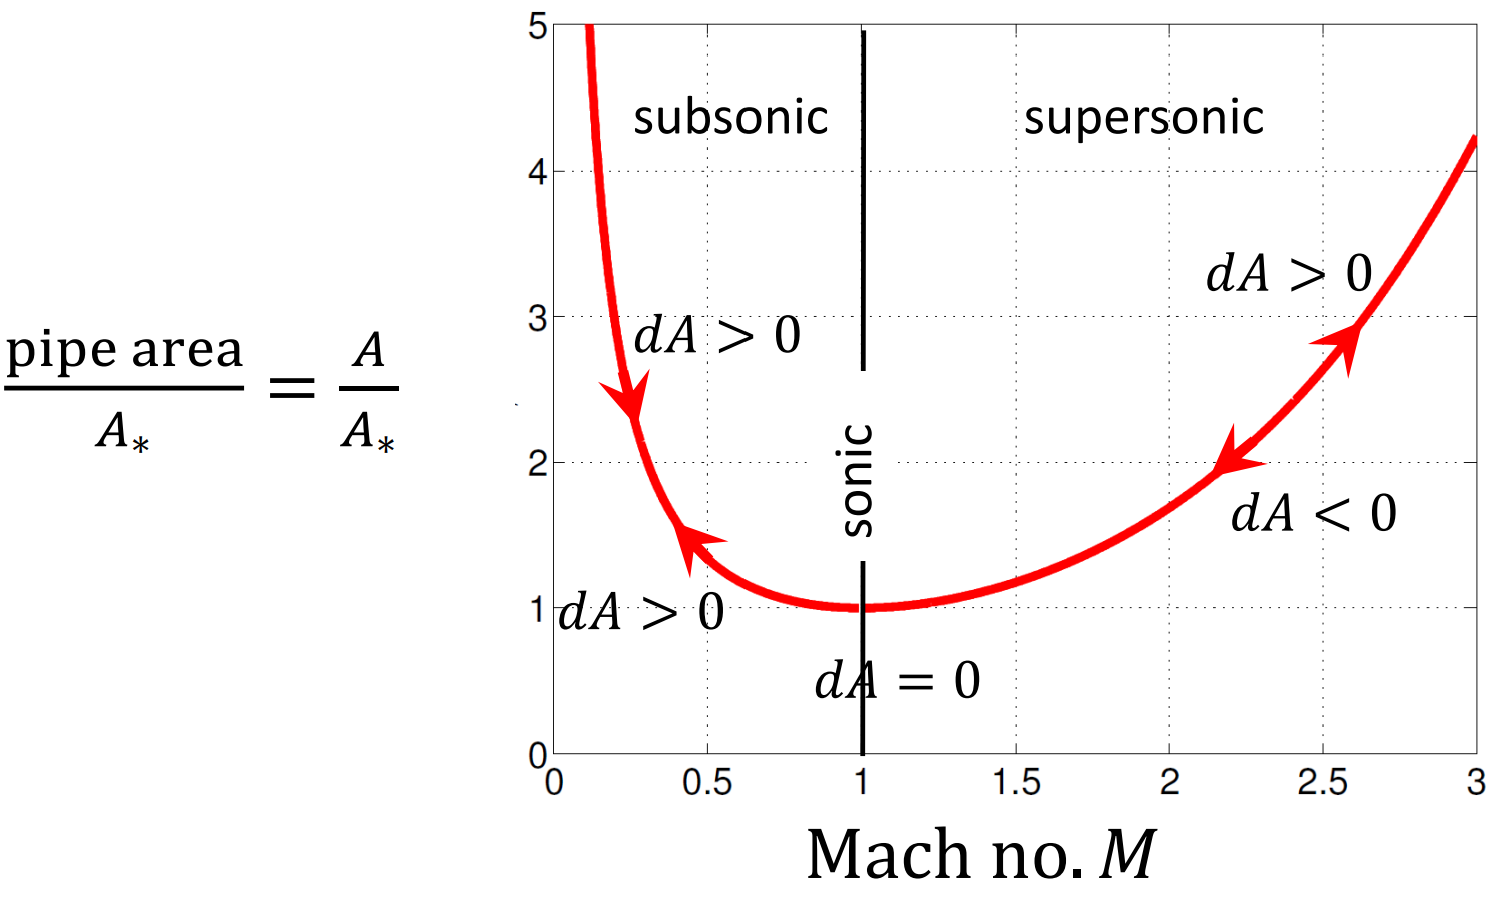
\includegraphics[width = 0.8 \textwidth]{../img/diagram52.png}
  \caption{Formation of a vortex, due to flow separation and flow reversal.}
\end{figure}
Favourable pressure gradient:
\begin{align}
  \frac{\partial U(x)}{\partial x} > 0, \ \frac{\partial p}{\partial x} <0
\end{align}
Adverse pressure gradient:
\begin{align}
  \frac{\partial U(x)}{\partial x} < 0, \ \frac{\partial p}{\partial x} > 0
\end{align}
Adverse pressure gradient produces further retardation of fluid (which is already slowed down close to wall). The fluid near to the wall is eventually brought to rest, flow reverse and separated. Separation occurs at or near the point where $\frac{dp}{dx}$ first becomes zero; at the first point of separation, at $y = 0$, $\frac{du}{dy} =0$. The formation of separation occurs as the fluid accelerates from the centre to get round the cylinder (it must accelerate as it has further to go than the surround fluid). It reaches a maximum at $Y-Y$, where it has also dropped in pressure. The adverse pressure gradient between here and the downstream side of the cylinder will cause separation if the flow is fast enough ($Re > 2$).
\begin{figure}[H]
  \centering
  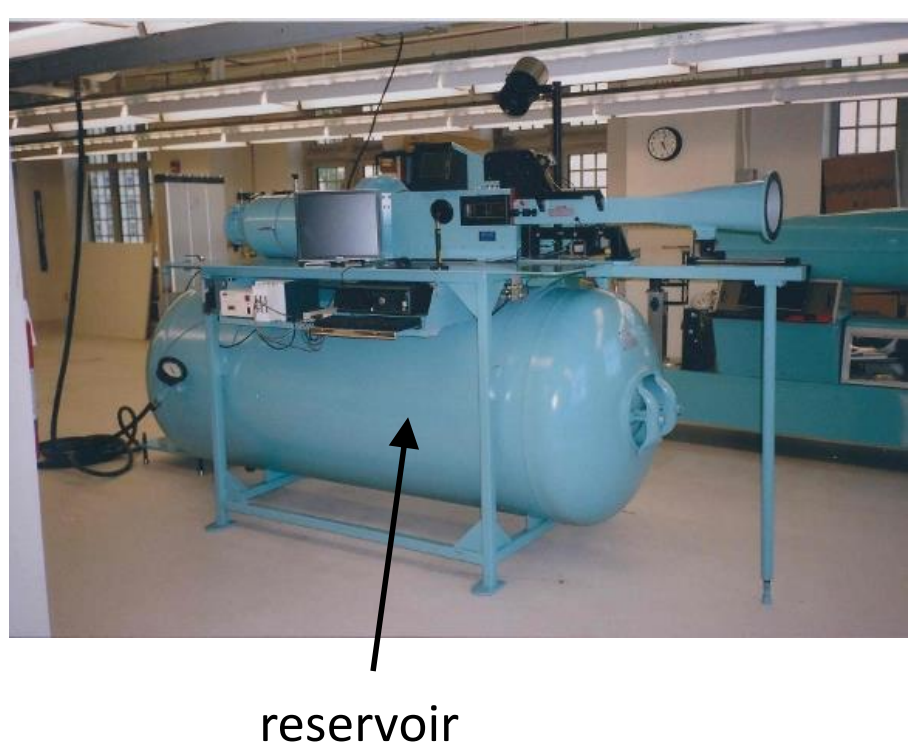
\includegraphics[width = 0.6 \textwidth]{../img/diagram53.png}
\end{figure}
\section{Laminar and turbulent flow separation}
\begin{figure}[H]
  \centering
  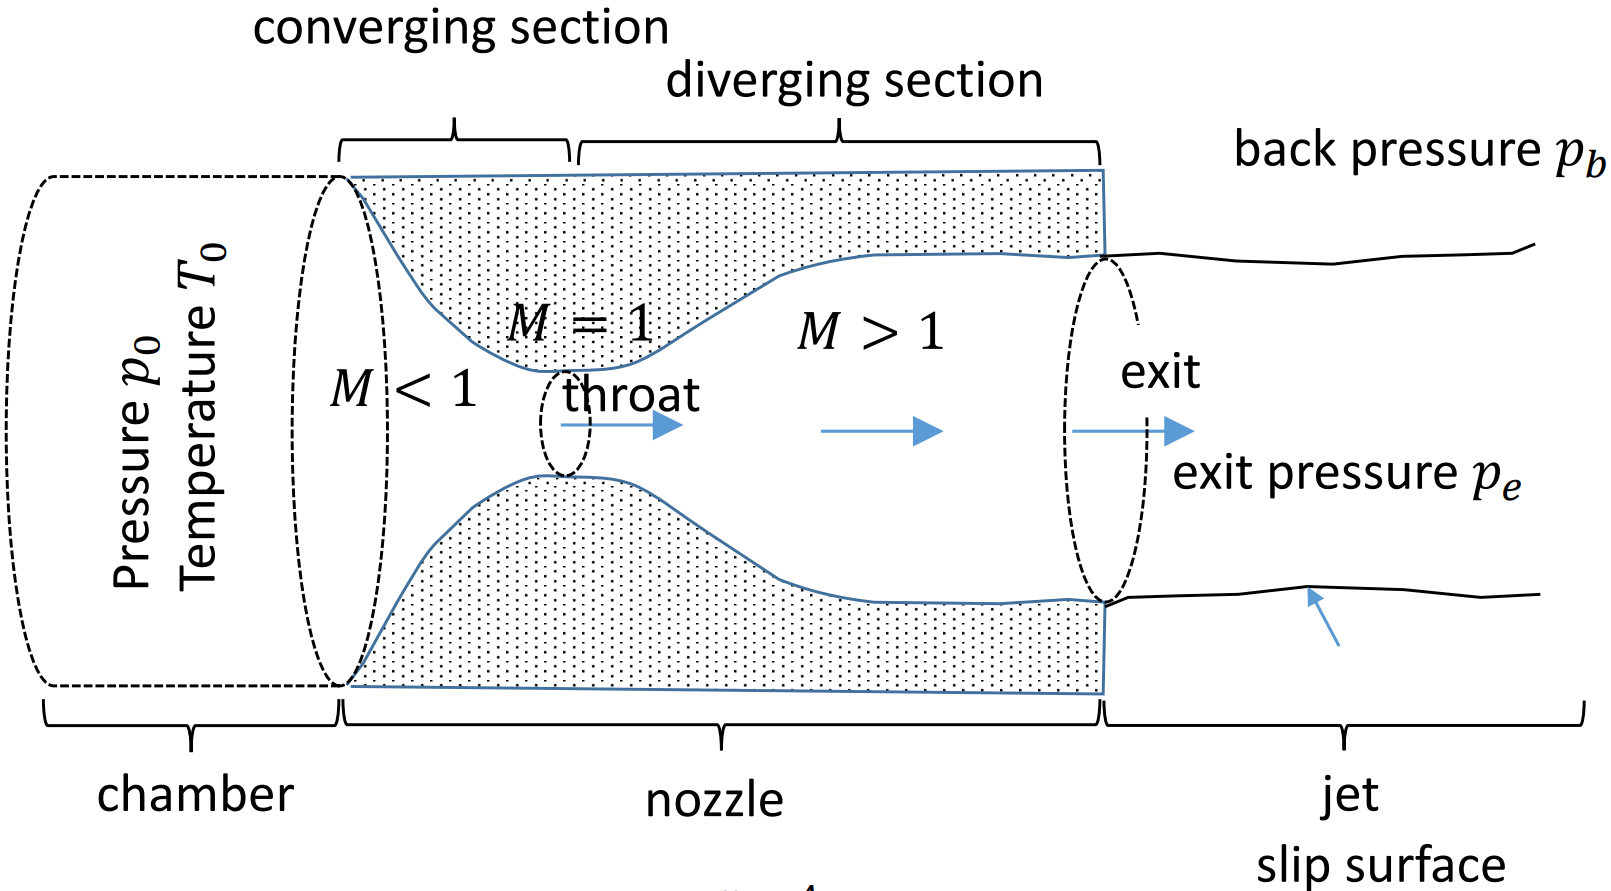
\includegraphics[width = 0.6 \textwidth]{../img/diagram54.png}
  \caption{Left: laminar, right: turbulent}
\end{figure}
The boundary layer has a high momentum deficit and in the case of laminar flow, it is unable to adjust to the increasing pressure and separates. A turbulent boundary layer is more resistant to separation than a laminar one. Due to the chaotic nature of turbulence, a turbulent boundary layer has a great capacity for mixing and absorbing energy from the free stream (this is obvious from its profile and its rate of growth compared with a laminar layer). The effect of increased mixing is increased transport of momentum (due to turbulent stresses) between the free-stream and the flow near the wall. This increased transport of momentum from the free-stream to the wall increases the stream-wise momentum in the boundary layer allowing the flow to overcome $\frac{dp}{dx}$ for longer and to separate further downstream (larger velocities near the wall are not so easily halted). 
\begin{figure}[H]
  \centering
  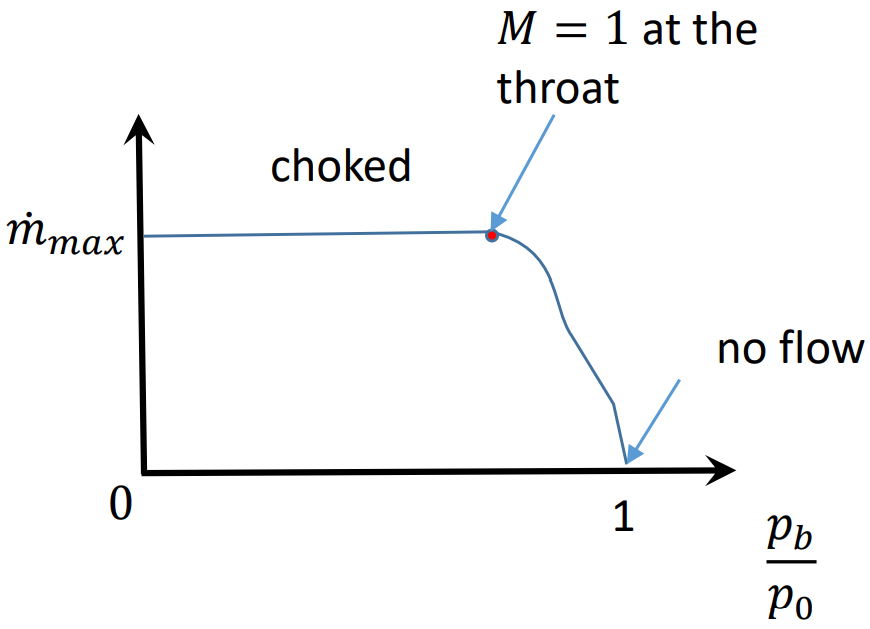
\includegraphics[width = \textwidth]{../img/diagram55.png}
\end{figure}
\section{Flow past a cylinder - Drag coefficient}
\begin{figure}[H]
  \centering
  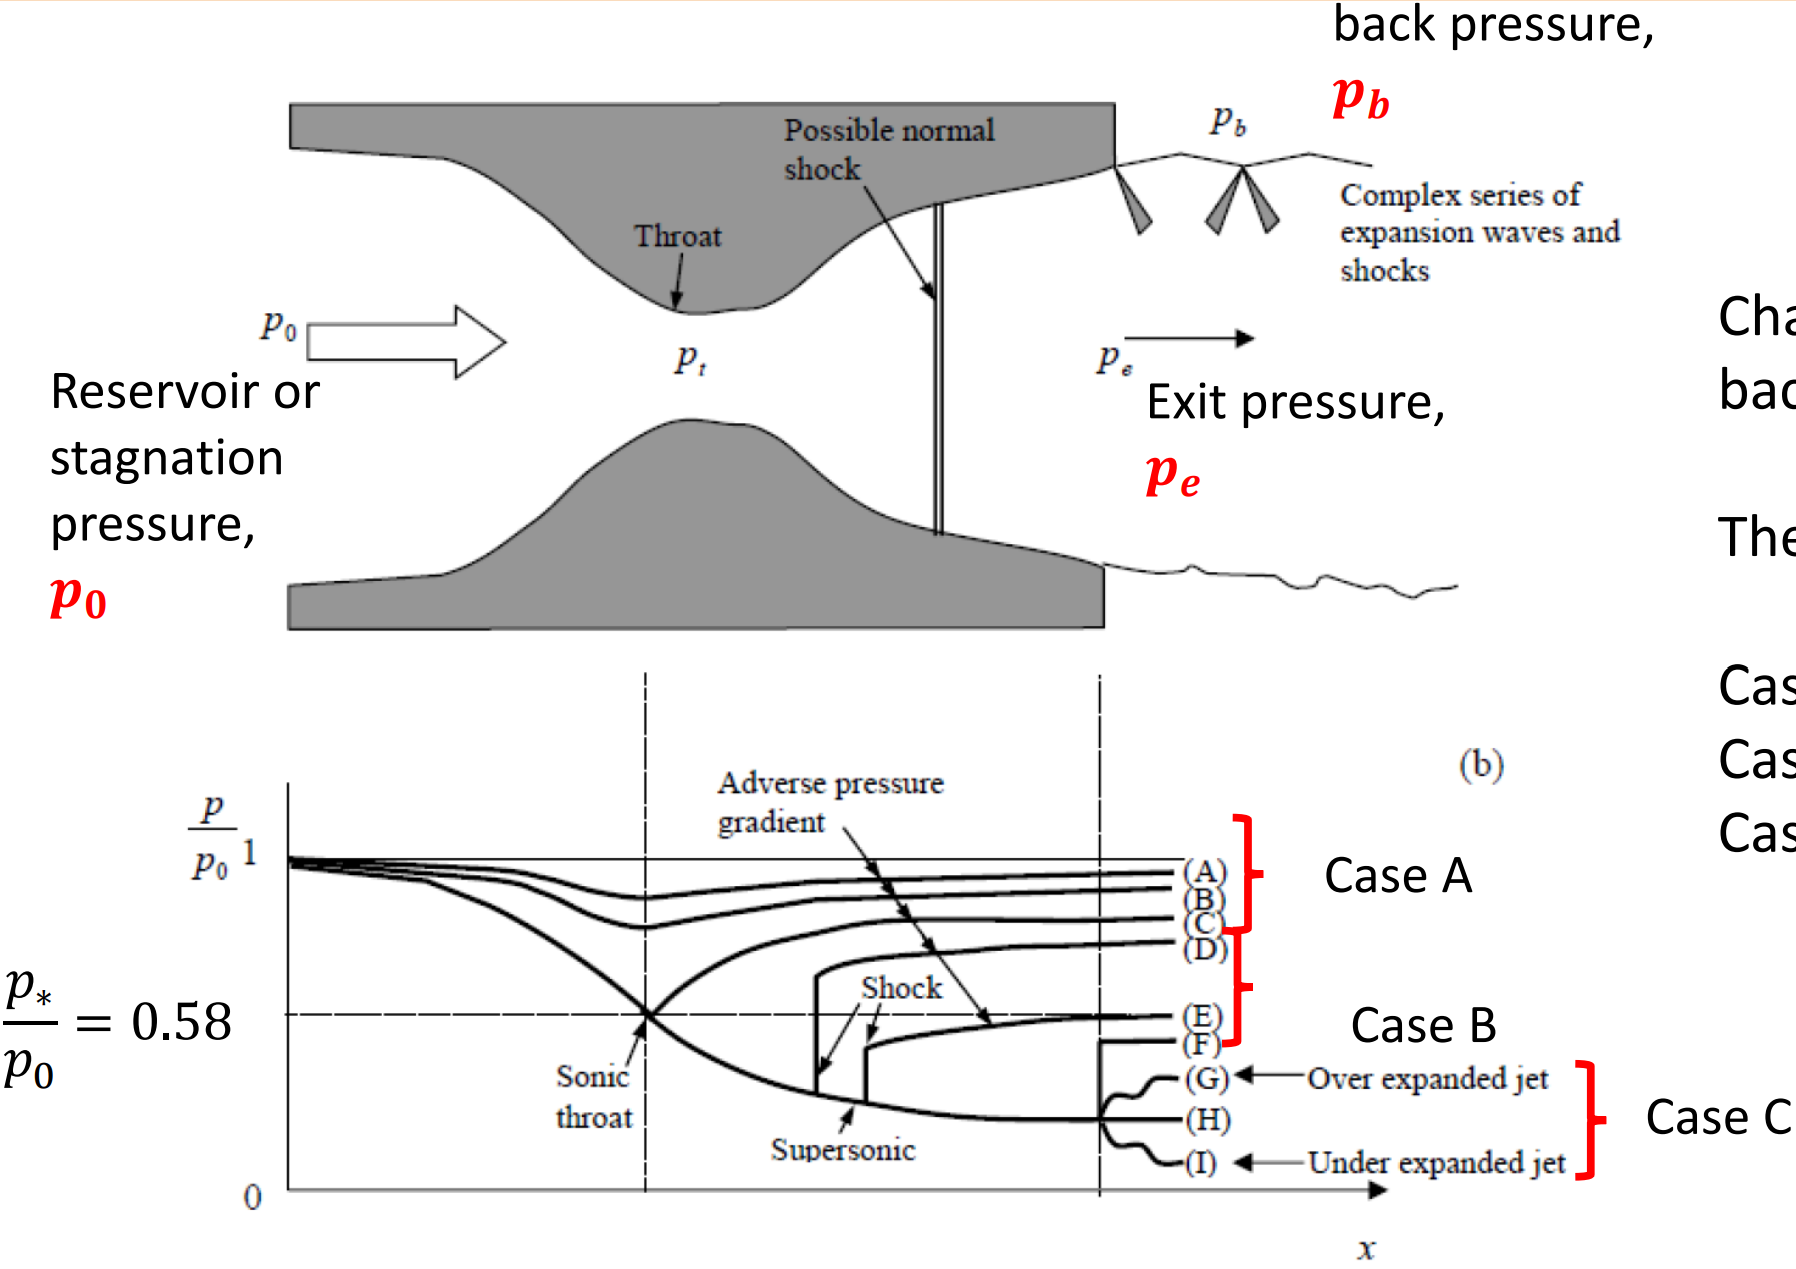
\includegraphics[width = 0.8\textwidth]{../img/diagram56.png}
\end{figure}
For a cylinder, 
\begin{itemize}
  \item $c_D$ is nearly constant when $Re = 10^3 - 10^5$, but varies considerably as the boundary layer becomes turbulent between $Re = 10^5 - 10^6$
  \item At $Re \approx 2000$, $c_D$ reaches minimum of $\approx 0.9$
  \item At $Re \approx 30000$, $c_D$ rises to $\approx 1.2$ (partly due to increasing turbulence in the wake)
  \item At $Re \approx 200000$, $c_D$ drops suddenly to $\approx 0.3$
  \item At $Re > 200000$, $c_D$ increases slowly. 
  \item The form drag is $\approx 50\%$ of the profile drag as $Re \rightarrow 0$
  \item By $Re \approx 200$ the form drag is $\approx 90\%$ of the profile drag
  \item At $Re \approx 30000$, skin friction is insignificant.
\end{itemize}
\section{Flow past a sphere}
The flow over a sphere starts to separate from the surface at $Re \approx 20$. As $Re$ increases, a pair of recirculating vortices becomes visible in the wake region. At flows up to $Re \approx 200$ the flow is still steady but beyond this value oscillations start to appear and the separation point moves upstream of the top of the sphere, increasing the drag. 
\begin{figure}[H]
  \centering
  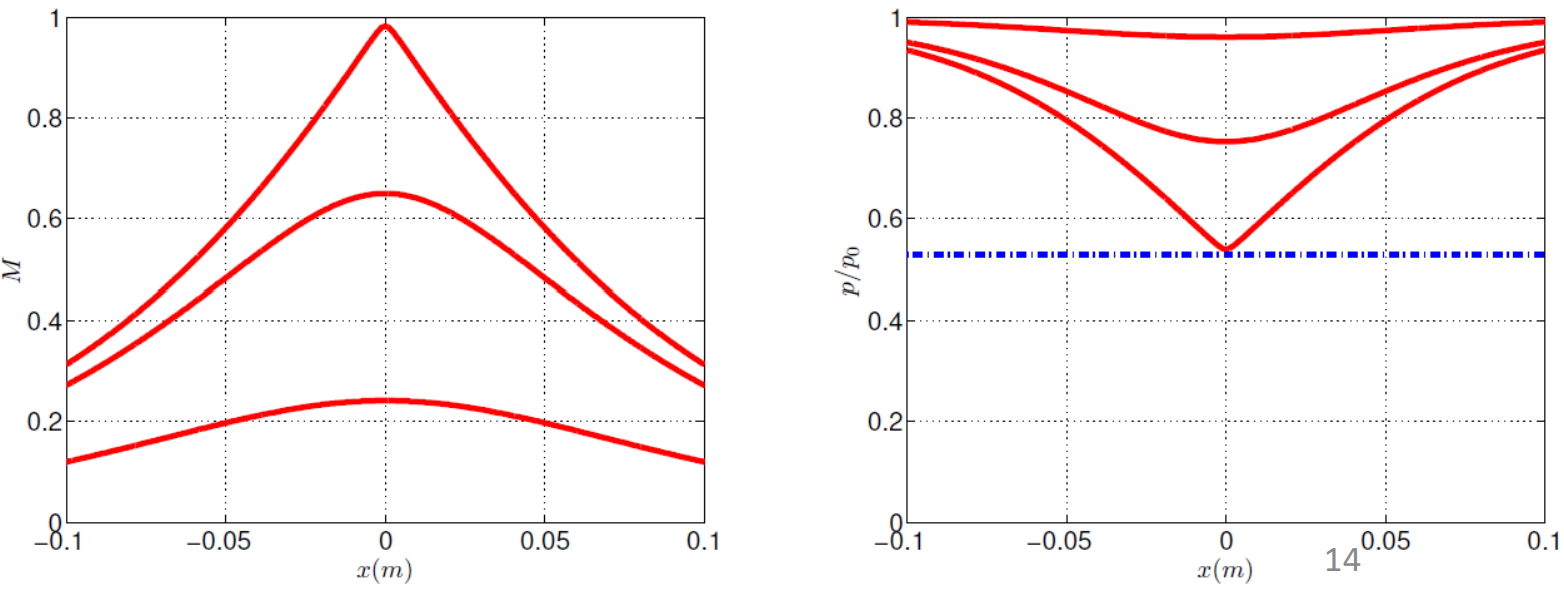
\includegraphics[width = \textwidth]{../img/diagram57.png}
\end{figure}
\subsection{Drag coefficient}
\begin{figure}[H]
  \centering
  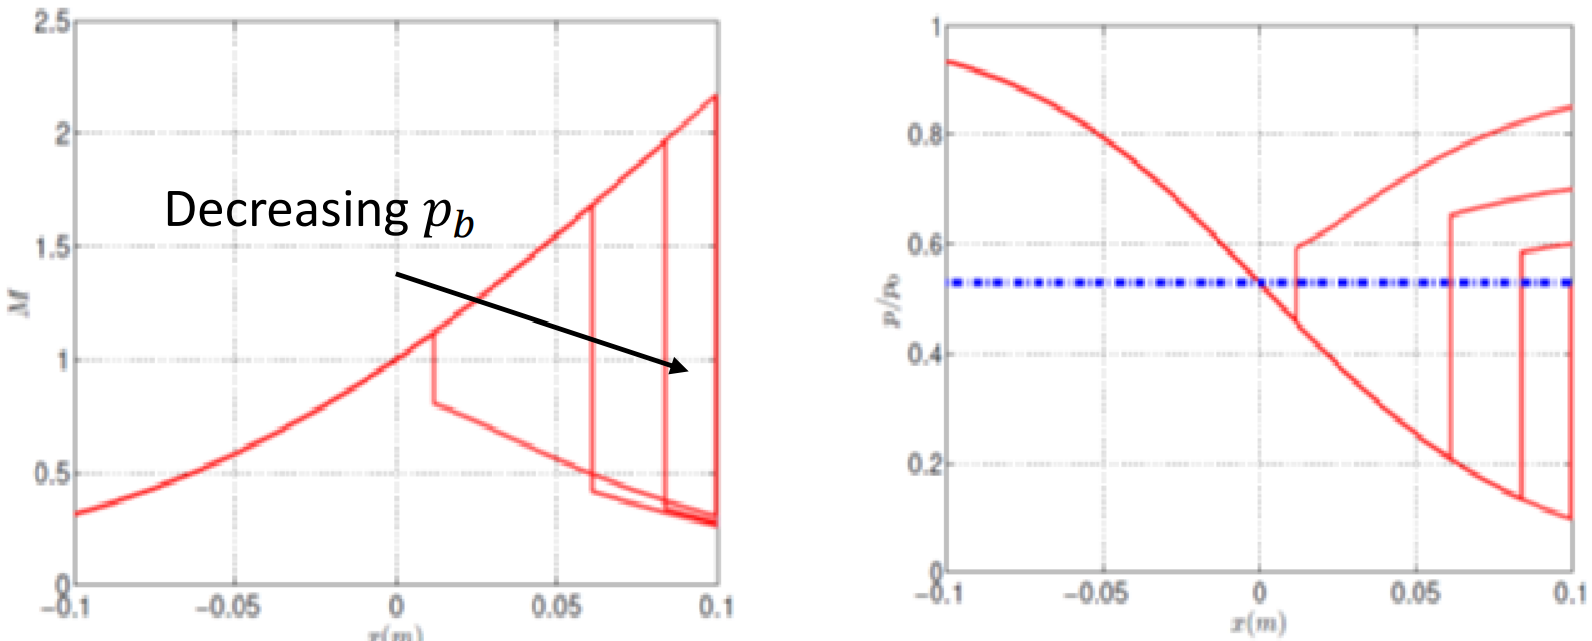
\includegraphics[width = 0.8\textwidth]{../img/diagram58.png}
\end{figure}
For a sphere, $c_D$ is nearly constant for $Re = 10^3 - 10^5$ but varies considerably as the boundary layer becomes turbulent between $Re = 10^5 - 10^6$ and, in fact, this transition causes $c_D$ to dramatically decrease. As $Re \rightarrow 0$, $c_D$ is given by Stokes's law ($c_D = \frac{24}{Re}$)
\subsection{Drag reduction}
Deliberately tripping the boundary layer from laminar to turbulent (i.e. by a trip wire) results in an increase in skin drag (due to increased shear stresses), but a decrease in form drag (due to delayed separation point). The reduction in form drag more than compensates for the increased drag due to turbulent shearing, resulting in a greatly reduced overall drag coefficient $c_D$. Drag reduction can also be accomplished by roughening the surface and, thereby, lowering $Re$ at which transition occurs. However, the drag coefficient for a roughened surface will typically rise faster in comparison to a smooth surface, once the transition point is passed. 
\begin{figure}[H]
  \centering
  \includegraphics[width = \textwidth]{../img/diagram59.png}
\end{figure}
\section{Flow past an aerofoil - stalling}
If the angle of attack becomes too great and boundary layer separation occurs on top of the aerofoil, the pressure pattern will change dramatically. In such a case, the lift component is insufficient to overcome the weight of one aircraft and disaster is imminent. This phenomenon is known as \textbf{stalling}. When stalling occurs, all, or most, of the 'suction' pressure is lost, and the plane will suddenly drop from the sky. The solution to this is to put the plane into a dive to regain the boundary layer. A transverse lift force is then exerted on the wing which gives the pilot some control and allows the plane to be pulled out of the dive.
\begin{figure}[H]
  \centering
  \includegraphics[width = \textwidth]{../img/diagram60.png}
\end{figure}
\begin{figure}[H]
  \centering
  \includegraphics[width =0.7 \textwidth]{../img/diagram61.png}
\end{figure}
\section{Boundary layer control}
There are mechanisms for preventing the boundary layer from separating in the first place.
\begin{itemize}
  \item Surface roughening
  \begin{itemize}
    \item To initiate turbulent boundary layer, thus delay separation and achieve a narrower wake of higher pressure
  \end{itemize}
  \item Shape variation
  \begin{itemize}
    \item Putting a flap at the end of the wing and tilting it before separation occurs increases the velocity over the top of the wing, reduces the pressure and chance of separation 
  \end{itemize}
  \item Fluid injection
  \begin{itemize}
    \item Accelerate boundary layer in direction of flow (but this will produce very turbulent flow and more skin friction)
  \end{itemize}
  \item Fluid removal
  \begin{itemize}
    \item Suction through small holes or a porous surface
    \item Downstream of suction position, boundary layer is thinner and faster thus better able to withstand adverse pressure gradient. Suction delays laminar to turbulent transition and leads to less skin friction
  \end{itemize}
  \item Slotted wing
  \begin{itemize}
    \item Slower moving air on the upper surface can be accelerated by bringing air from the high-pressure area on the bottom of the wing through slots. Pressure decreases on the top and adverse pressure gradient reduces
  \end{itemize}
  \item Engine arrangement
  \begin{itemize}
    \item Engine intakes draw slow air from the boundary layer at the rear of the wing through small holes. This keeps the boundary layer close to the wing and greater pressure gradients can be maintained before separation
  \end{itemize}
\end{itemize}
Control systems are often costly and difficult to install. Advantages for some conditions, hindrance of others (advantages maybe offset by the added drag). Planes take advantage of the cambered aerofoil's high lift characteristics by enabling shape variation of the basic wing. Leading edge 'Krüger' flaps or slats and trailing edge 'Fowler' flaps are extended from the wing and change the aerofoil's shape into a cambered form, generating greater lift during low-speed flight.
\begin{figure}[H]
  \centering
  \includegraphics[width =0.5 \textwidth]{../img/diagram63.png}
\end{figure}
\begin{figure}[H]
  \centering
  \includegraphics[width =0.8 \textwidth]{../img/diagram62.png}
\end{figure}
\begin{figure}[H]
  \centering
  \includegraphics[width =0.7 \textwidth]{../img/diagram64.png}
\end{figure}
\begin{figure}[H]
  \centering
  \includegraphics[width =0.7 \textwidth]{../img/diagram65.png}
\end{figure}
\begin{figure}[H]
  \centering
  \includegraphics[width =0.7 \textwidth]{../img/diagram66.png}
\end{figure}
\end{document}